
%(BEGIN_QUESTION)
% Copyright 2008, Tony R. Kuphaldt, released under the Creative Commons Attribution License (v 1.0)
% This means you may do almost anything with this work of mine, so long as you give me proper credit

Calculate and superimpose two {\it load lines} for this circuit on top of the transistor's characteristic curves, one load line for $R_{load}$ = 2 k$\Omega$ and another one for $R_{load}$ = 4 k$\Omega$:

$$\includegraphics[width=15.5cm]{i03224x01.eps}$$

Next, calculate the amount of collector current in the two different circuits (with different $R_{load}$ values) at the following base current values:

% No blank lines allowed between lines of an \halign structure!
% I use comments (%) instead, so that TeX doesn't choke.

$$\vbox{\offinterlineskip
\halign{\strut
\vrule \quad\hfil # \ \hfil & 
\vrule \quad\hfil # \ \hfil & 
\vrule \quad\hfil # \ \hfil \vrule \cr
\noalign{\hrule}
%
% First row
Base current & Collector current & Collector current \cr
%
($I_B$) & ($I_C$) $R_{load}$ = 2 k$\Omega$ & ($I_C$) $R_{load}$ = 4 k$\Omega$\cr
%
\noalign{\hrule}
%
% Another row
0 $\mu$A &  &  \cr
%
\noalign{\hrule}
%
% Another row
10 $\mu$A &  &  \cr
%
\noalign{\hrule}
%
% Another row
20 $\mu$A &  &  \cr
%
\noalign{\hrule}
%
% Another row
30 $\mu$A &  &  \cr
%
\noalign{\hrule}
%
% Another row
40 $\mu$A &  &  \cr
%
\noalign{\hrule}
} % End of \halign 
}$$ % End of \vbox

Looking at the relationship between $I_B$ and $I_C$ now, which of these two circuits yields the more {\it linear} response?  In other words, for which load resistor value does the transistor exhibit the most proportional response to increases in base current?  Explain why.

\underbar{file i03224}
%(END_QUESTION)





%(BEGIN_ANSWER)

$$\includegraphics[width=15.5cm]{i03224x02.eps}$$

% No blank lines allowed between lines of an \halign structure!
% I use comments (%) instead, so that TeX doesn't choke.

$$\vbox{\offinterlineskip
\halign{\strut
\vrule \quad\hfil # \ \hfil & 
\vrule \quad\hfil # \ \hfil & 
\vrule \quad\hfil # \ \hfil \vrule \cr
\noalign{\hrule}
%
% First row
Base current & Collector current & Collector current \cr
%
($I_B$) & ($I_C$) $R_{load}$ = 2 k$\Omega$ & ($I_C$) $R_{load}$ = 4 k$\Omega$\cr
%
\noalign{\hrule}
%
% Another row
0 $\mu$A & 0.5 mA & 0.5 mA \cr
%
\noalign{\hrule}
%
% Another row
10 $\mu$A & 3.9 mA & 3.4 mA \cr
%
\noalign{\hrule}
%
% Another row
20 $\mu$A & 6.5 mA & 5.0 mA \cr
%
\noalign{\hrule}
%
% Another row
30 $\mu$A & 9.0 mA & 5.3 mA \cr
%
\noalign{\hrule}
%
% Another row
40 $\mu$A & 10.2 mA & 5.4 mA \cr
%
\noalign{\hrule}
} % End of \halign 
}$$ % End of \vbox

Less load resistance yields the most linear $I_C$-versus-$I_B$ response from the transistor, because it is with a lower load resistance that the voltage across the transistor ($V_{CE}$) is the most stable.  Increased load resistance ``starves'' the transistor of voltage at higher current values.

%(END_ANSWER)





%(BEGIN_NOTES)

It would be good to point out something here: superimposing a linear function on a set of nonlinear functions and looking for the intersection points allows us to solve for multiple variables in a nonlinear mathematical system.  Normally, only {\it linear} systems of equations are considered ``solvable'' without resorting to very time-consuming arithmetic computations, but here we have a powerful (graphical) tool for approximating the values of variables in a nonlinear system.  Since approximations are the best we can hope for in transistor circuits anyway, this is good enough!

%INDEX% Electronics review: load lines
%INDEX% Final Control Elements, valve: characterization

%(END_NOTES)


